Un des intérêts principaux de LaTeX est sa gestion
formidable des mathématiques.
Il est donc important de savoir comment écrire des formules mathématiques.
C'est l'objet de cette section.

\subsection{Les mathématiques en LaTeX}\label{subsec:latex_math}

LaTeX est particulièrement adapté pour écrire des formules mathématiques.
Qu'elles soient simples comme

\begin{equation}
    a + b = c
\end{equation}

ou bien plus farfelues comme

\begin{equation}\label{eq:2}
\boxed{
\frac{\partial^2 \Psi}{\partial t^2} = c^2 \nabla^2 \Psi + \underbrace{\sum_{k=1}^n \left( \frac{\hbar^2}{2m_k} \int_{\Omega} |\nabla \psi_k|^2 d^3\mathbf{r} \right)}_{\text{Quantum Potential Terms}} - \overbrace{\bigotimes_{j=1}^m \begin{pmatrix}
\alpha_j & -\beta_j^* \\
\beta_j & \alpha_j^*
\end{pmatrix}}^{\text{Unitary Operators}} + \left[ \prod_{i=1}^\infty \frac{p_i^{s_i}}{1-p_i^{-s_i}} \right]
}
\end{equation}

ou bien encore

\begin{equation}\label{eq:3}
\iiint\limits_{\mathcal{V}} \left( \frac{\rho\mathbf{v} \cdot \mathbf{v}}{2} + \rho e \right) dV = \oint_{\partial \mathcal{V}} \mathbf{T} \cdot \mathbf{v} \, dA + \underbrace{\int_{\mathcal{V}} \rho \mathbf{f} \cdot \mathbf{v} \, dV + \dot{Q}}_{\text{External Work and Heat}} - \frac{d}{dt} \left( \frac{1}{2} \sum_{\substack{i,j=1 \\ i\neq j}}^{N} \frac{G m_i m_j}{|\mathbf{r}_i - \mathbf{r}_j|} \right)
\end{equation}

LaTeX permet d'écrire des formules mathématiques de manière très élégante.
Ne vous inquiétez pas, vous n'aurez pas besoin de savoir écrire des formules aussi compliquées
mais il est utile d'en connaître certains éléments.

\subsection{Les 2 modes d'écriture}\label{subsec:latex_math_modes}

Il existe deux manières principales d'écrire des formules mathématiques en LaTeX:\@

\begin{itemize}
    \item \textbf{Inline math mode}: C'est le mode par défaut pour écrire des formules mathématiques dans le texte.
    Il ressemble à ceci: \(a + b = c\) et s'écrit entre des signes \texttt{\textbackslash( \(\cdot\) \textbackslash)}

    \item \textbf{Display math mode}: C'est le mode pour écrire des formules mathématiques plus grandes et plus complexes.
    Il ressemble à ceci:
    \begin{equation}
        \int_0^1 x^2 \, dx = \frac{1}{3}
    \end{equation}
    et s'écrit entre des signes \texttt{\textbackslash[ \(\cdot\) \textbackslash]} ou 
    dans un environnement mathématique comme \texttt{equation}.
\end{itemize}

Il est important de savoir qu'il vaut mieux éviter d'utiliser le mode inline
pour écrire des formules mathématiques trop longues ou trop complexes. Comme l'indique son nom,
le mode inline est fait pour écrire des formules mathématiques courtes et simples dans le texte.

Il est une bonne pratique d'utiliser le mode display pour écrire des grosses formules
mathématiques ou des formules qui prennent plusieurs lignes.

\subsection{Les symboles mathématiques}\label{subsec:latex_math_symbols}
Il existe de très nombreux symboles mathématiques en LaTeX.
Il vaut mieux utiliser le site \href{detexify.kirelabs.org}{Detexify} pour
trouver le symbole que vous cherchez à partir d'un dessin ou alors se référer à la
documentation de LaTeX (le site est vraiment très fort). Je vous en donne quand même quelques uns ici:

% image of the site working well
\begin{figure}[H]
    \centering
    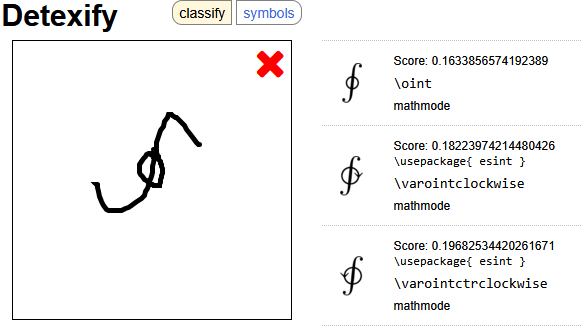
\includegraphics[width=0.5\textwidth]{./4_Mathematics/detexify}
    \caption{Le site Detexify}\label{fig:detexify}
\end{figure}

\begin{itemize}
    \item \textbf{Les symboles de base}:
    \begin{itemize}
        \item \texttt{\textbackslash{}geq} pour \(\geq\)
        \item \texttt{\textbackslash{}infty} pour \(\infty\)
        \item \texttt{\textbackslash{}exists} pour \(\exists\)
        \item \texttt{\textbackslash{}int} pour \(\int\)
        \item \texttt{\textbackslash{}sum} pour \(\sum\)
        \item Encore une fois, il est facile de deviner le nom de la commande
    \end{itemize}
    \item \textbf{Les symboles de logique}:
    \begin{itemize}
        \item \texttt{\textbackslash{}land} pour \(\land\)
        \item \texttt{\textbackslash{}lor} pour \(\lor\)
        \item Remarquez que c'est simplement le nom anglais précédée de \texttt{\textbackslash{}l}
    \end{itemize}
    \item \textbf{Les environnements mathématiques}:
    \begin{itemize}
        \item \texttt{\textbackslash{}begin\{equation\}} et \texttt{\textbackslash{}end\{equation\}} pour écrire une équation
        \item \texttt{\textbackslash{}begin\{align\}} et \texttt{\textbackslash{}end\{align\}} pour écrire une équation alignée
        \item Si vous ne voulez pas d'équation numérotée, rajoutez un \texttt{*} à la fin de l'environnement
        \item Par exemple, \texttt{\textbackslash{}begin\{equation*\}} et \texttt{\textbackslash{}end\{equation*\}}
    \end{itemize}
\end{itemize}

\subsection{Les choses à savoir}\label{subsec:latex_math_know}

Vous avez sûrement remarqué que dans les équations~\eqref{eq:2} et~\eqref{eq:3},
il y a des éléments qui ne ressemblent pas à des simples symboles. En effet,
on peut faire plus que simplement écrire des symboles mathématiques en LaTeX.
Il est possible de faire des choses comme:
\begin{itemize}
    \item \textbf{Mettre une boîte autour d'une formule} avec \texttt{\textbackslash{}boxed\{\(\cdots\)\}}:
    \begin{equation}
        \boxed{a + b = c}
    \end{equation}
    \item \textbf{Mettre une barre autour d'une formule} avec \texttt{\textbackslash{}overline\{\(\cdots\)\}}:
    \begin{equation}
        \overline{a + b = c}
    \end{equation}
    \item \textbf{Mettre une parenthèse autour d'une formule} avec \texttt{\textbackslash{}left( \(\cdots\) \textbackslash{}right)}:
    \begin{equation}
        \left( a + b = c \right)
    \end{equation}
    \item \textbf{Ecrire en dessous d'une formule} avec \texttt{\textbackslash{}underbrace\{\(\cdots\)\}\textunderscore\{\(\cdots\)\}}:
    \begin{equation}
        \underbrace{a + b = c}_{\text{C'est une équation}}
    \end{equation}
    \item \textbf{Indicer à plusieurs niveaux} avec \texttt{\textbackslash{}substack\{\(\cdots\)\}}:
    \begin{equation}
        \sum_{\substack{i=1 \\ j=2}}^{n} i + j
    \end{equation}
\end{itemize}

Bien plus est encore possible mais cela vient en recherchant dans la documentation
et avec le temps. Un conseil est de ne pas hésiter à regarder le code source
d'un document LaTeX pour le comprendre ou y piocher des éléments cools.

\subsection{Les environnements spécialisés}\label{subsec:latex_math_env}

Latex propose en plus des environnements mathématiques précédents des environnements 
supplémentaires permettant la définition d'environnement comme les théorèmes, les exemples etc

Je vous conseille d'aller voir directement la documentation du package \texttt{amsthm}
car il est très complet et je ne vais pas le détailler ici.

\subsection{Le référencement}\label{subsec:latex_math_ref}

Si vous avez été curieux, vous avez essayé de cliquer sur les références
~\eqref{eq:2} et~\eqref{eq:3} et avez été émerveillé de voir que
cela vous a amené directement à l'équation en question.
C'est cela qu'on appelle le référencement.

On peut référencer des équations, des sections, des figures, des tableaux,
des théorèmes, des définitions, etc. On peut référencer tout ce qu'on veut
en LaTeX. Il suffit de faire ceci:
\begin{enumerate}
    \item Rajouter une \texttt{\textbackslash{}label\{\(\cdots\)\}} à l'endroit
    où vous voulez référencer l'élément. Il lui faut un nom unique.
    \item Utiliser la commande \texttt{\textbackslash{}ref\{\(\cdots\)\}} pour
    référencer l'élément.
    \item Si vous voulez référencer une équation, utilisez \texttt{\textbackslash{}eqref\{\(\cdots\)\}}.
\end{enumerate}

Attention, ce référencement est différent de celui qu'on utilise
dans les bibliographies. Il ne faut pas confondre les deux.